\documentclass[a4paper,10pt]{article}
\usepackage[utf8]{inputenc}
\usepackage[T1]{fontenc}
\usepackage[francais]{babel}
\usepackage[a4paper,top=2.5cm, bottom=2.5cm, left=2.5cm, right=2.5cm]{geometry}
\usepackage{longtable}
\usepackage[final]{pdfpages} 


%opening
\title{INFO-F-403 : Language theory and compiling \\ Rapport projet partie 2 - Grammaire}
\author{Simon Picard \\ Arnaud Rosette}

\begin{document}

\maketitle

\section{Grammaire}

\begin{longtable}{llll}
$[1]$&<Program>&$\rightarrow$&\begin{tabular}[t]{@{}l@{}}<InstructionList> \end{tabular}\\
$[2]$&<InstructionList>&$\rightarrow$&\begin{tabular}[t]{@{}l@{}}<IdentifierInstruction> \\END\_OF\_INSTRUCTION <InstructionList> \end{tabular}\\
$[3]$&&$\rightarrow$&\begin{tabular}[t]{@{}l@{}}<ConstDefinition> END\_OF\_INSTRUCTION \\<InstructionList> \end{tabular}\\
$[4]$&&$\rightarrow$&\begin{tabular}[t]{@{}l@{}}<Block> END\_OF\_INSTRUCTION \\<InstructionList> \end{tabular}\\
$[5]$&&$\rightarrow$&\begin{tabular}[t]{@{}l@{}}<Loop> END\_OF\_INSTRUCTION \\<InstructionList> \end{tabular}\\
$[6]$&&$\rightarrow$&\begin{tabular}[t]{@{}l@{}}<BuiltInFunctionCall> END\_OF\_INSTRUCTION \\<InstructionList> \end{tabular}\\
$[7]$&&$\rightarrow$&\begin{tabular}[t]{@{}l@{}}<FunctionDefinition> END\_OF\_INSTRUCTION \\<InstructionList> \end{tabular}\\
$[8]$&&$\rightarrow$&\begin{tabular}[t]{@{}l@{}}END\_OF\_INSTRUCTION <InstructionList> \end{tabular}\\
$[9]$&&$\rightarrow$&\begin{tabular}[t]{@{}l@{}}EPSILON\_VALUE \end{tabular}\\
$[10]$&<IdentifierInstruction>&$\rightarrow$&\begin{tabular}[t]{@{}l@{}}IDENTIFIER <IdentifierInstructionTail> \end{tabular}\\
$[11]$&<IdentifierInstructionTail>&$\rightarrow$&\begin{tabular}[t]{@{}l@{}}<AssignationTail> \end{tabular}\\
$[12]$&&$\rightarrow$&\begin{tabular}[t]{@{}l@{}}TYPE\_DEFINITION <Type> \end{tabular}\\
$[13]$&&$\rightarrow$&\begin{tabular}[t]{@{}l@{}}<FunctionCallTail> \end{tabular}\\
$[14]$&<AssignationTail>&$\rightarrow$&\begin{tabular}[t]{@{}l@{}}ASSIGNATION <Expression> \end{tabular}\\
$[15]$&&$\rightarrow$&\begin{tabular}[t]{@{}l@{}}COMMA IDENTIFIER <AssignationTail> COMMA \\<Expression> \end{tabular}\\
$[16]$&<ConstDefinition>&$\rightarrow$&\begin{tabular}[t]{@{}l@{}}CONST IDENTIFIER <AssignationTail> \end{tabular}\\
$[17]$&<Block>&$\rightarrow$&\begin{tabular}[t]{@{}l@{}}LET IDENTIFIER <AssignationTail> \\END\_OF\_INSTRUCTION <InstructionList> END \end{tabular}\\
$[18]$&<Loop>&$\rightarrow$&\begin{tabular}[t]{@{}l@{}}<If> \end{tabular}\\
$[19]$&&$\rightarrow$&\begin{tabular}[t]{@{}l@{}}WHILE <Expression> END\_OF\_INSTRUCTION \\<InstructionList> END \end{tabular}\\
$[20]$&&$\rightarrow$&\begin{tabular}[t]{@{}l@{}}FOR IDENTIFIER ASSIGNATION <Expression> \\TERNARY\_ELSE <Expression> <ForTail> \end{tabular}\\
$[21]$&<ForTail>&$\rightarrow$&\begin{tabular}[t]{@{}l@{}}END\_OF\_INSTRUCTION <InstructionList> END \end{tabular}\\
$[22]$&&$\rightarrow$&\begin{tabular}[t]{@{}l@{}}TERNARY\_ELSE <Expression> \\END\_OF\_INSTRUCTION <InstructionList> END \end{tabular}\\
$[23]$&<Type>&$\rightarrow$&\begin{tabular}[t]{@{}l@{}}BOOLEAN\_TYPE \end{tabular}\\
$[24]$&&$\rightarrow$&\begin{tabular}[t]{@{}l@{}}REAL\_TYPE \end{tabular}\\
$[25]$&&$\rightarrow$&\begin{tabular}[t]{@{}l@{}}INTEGER\_TYPE \end{tabular}\\
$[26]$&<Expression>&$\rightarrow$&\begin{tabular}[t]{@{}l@{}}<BinaryExpression> <TernaryIfExpression> \end{tabular}\\
$[27]$&<TernaryIfExpression>&$\rightarrow$&\begin{tabular}[t]{@{}l@{}}TERNARY\_IF <Expression> \\<TernaryElseExpression> \end{tabular}\\
$[28]$&&$\rightarrow$&\begin{tabular}[t]{@{}l@{}}EPSILON\_VALUE \end{tabular}\\
$[29]$&<TernaryElseExpression>&$\rightarrow$&\begin{tabular}[t]{@{}l@{}}TERNARY\_ELSE <Expression> \end{tabular}\\
$[30]$&<AtomicExpression>&$\rightarrow$&\begin{tabular}[t]{@{}l@{}}<AtomicIdentifierExpression> \end{tabular}\\
$[31]$&&$\rightarrow$&\begin{tabular}[t]{@{}l@{}}INTEGER \end{tabular}\\
$[32]$&&$\rightarrow$&\begin{tabular}[t]{@{}l@{}}REAL \end{tabular}\\
$[33]$&&$\rightarrow$&\begin{tabular}[t]{@{}l@{}}BOOLEAN \end{tabular}\\
$[34]$&&$\rightarrow$&\begin{tabular}[t]{@{}l@{}}<BuiltInFunctionCall> \end{tabular}\\
$[35]$&<AtomicIdentifierExpression>&$\rightarrow$&\begin{tabular}[t]{@{}l@{}}IDENTIFIER \\<AtomicIdentifierExpressionTail> \end{tabular}\\
$[36]$&<AtomicIdentifierExpressionTail>&$\rightarrow$&\begin{tabular}[t]{@{}l@{}}<FunctionCallTail> \end{tabular}\\
$[37]$&&$\rightarrow$&\begin{tabular}[t]{@{}l@{}}EPSILON\_VALUE \end{tabular}\\
$[38]$&<UnaryExpression>&$\rightarrow$&\begin{tabular}[t]{@{}l@{}}NEGATION <UnaryExpression> \end{tabular}\\
$[39]$&&$\rightarrow$&\begin{tabular}[t]{@{}l@{}}<UnaryBitwiseNotExpression> \end{tabular}\\
$[40]$&<UnaryBitwiseNotExpression>&$\rightarrow$&\begin{tabular}[t]{@{}l@{}}BITWISE\_NOT <UnaryBitwiseNotExpression> \end{tabular}\\
$[41]$&&$\rightarrow$&\begin{tabular}[t]{@{}l@{}}<UnaryMinusPlusExpression> \end{tabular}\\
$[42]$&<UnaryMinusPlusExpression>&$\rightarrow$&\begin{tabular}[t]{@{}l@{}}MINUS <UnaryMinusPlusExpression> \end{tabular}\\
$[43]$&&$\rightarrow$&\begin{tabular}[t]{@{}l@{}}PLUS <UnaryMinusPlusExpression> \end{tabular}\\
$[44]$&&$\rightarrow$&\begin{tabular}[t]{@{}l@{}}<UnaryAtomicExpression> \end{tabular}\\
$[45]$&<UnaryAtomicExpression>&$\rightarrow$&\begin{tabular}[t]{@{}l@{}}<AtomicExpression> \end{tabular}\\
$[46]$&&$\rightarrow$&\begin{tabular}[t]{@{}l@{}}LEFT\_PARENTHESIS <Expression> \\RIGHT\_PARENTHESIS \end{tabular}\\
$[47]$&<BinaryExpression>&$\rightarrow$&\begin{tabular}[t]{@{}l@{}}<BinaryLazyOrExpression> \\<BinaryExpression'> \end{tabular}\\
$[48]$&<BinaryExpression'>&$\rightarrow$&\begin{tabular}[t]{@{}l@{}}LAZY\_OR <BinaryLazyOrExpression> \\<BinaryExpression'> \end{tabular}\\
$[49]$&&$\rightarrow$&\begin{tabular}[t]{@{}l@{}}EPSILON\_VALUE \end{tabular}\\
$[50]$&<BinaryLazyOrExpression>&$\rightarrow$&\begin{tabular}[t]{@{}l@{}}<BinaryLazyAndExpression> \\<BinaryLazyOrExpression'> \end{tabular}\\
$[51]$&<BinaryLazyOrExpression'>&$\rightarrow$&\begin{tabular}[t]{@{}l@{}}LAZY\_AND <BinaryLazyAndExpression> \\<BinaryLazyOrExpression'> \end{tabular}\\
$[52]$&&$\rightarrow$&\begin{tabular}[t]{@{}l@{}}EPSILON\_VALUE \end{tabular}\\
$[53]$&<BinaryLazyAndExpression>&$\rightarrow$&\begin{tabular}[t]{@{}l@{}}<BinaryNumericExpression> \\<BinaryLazyAndExpression'> \end{tabular}\\
$[54]$&<BinaryLazyAndExpression'>&$\rightarrow$&\begin{tabular}[t]{@{}l@{}}GREATER\_THAN <BinaryNumericExpression> \\<BinaryLazyAndExpression'> \end{tabular}\\
$[55]$&&$\rightarrow$&\begin{tabular}[t]{@{}l@{}}LESS\_THAN <BinaryNumericExpression> \\<BinaryLazyAndExpression'> \end{tabular}\\
$[56]$&&$\rightarrow$&\begin{tabular}[t]{@{}l@{}}GREATER\_OR\_EQUALS\_THAN \\<BinaryNumericExpression> \\<BinaryLazyAndExpression'> \end{tabular}\\
$[57]$&&$\rightarrow$&\begin{tabular}[t]{@{}l@{}}LESS\_OR\_EQUALS\_THAN \\<BinaryNumericExpression> \\<BinaryLazyAndExpression'> \end{tabular}\\
$[58]$&&$\rightarrow$&\begin{tabular}[t]{@{}l@{}}EQUALITY <BinaryNumericExpression> \\<BinaryLazyAndExpression'> \end{tabular}\\
$[59]$&&$\rightarrow$&\begin{tabular}[t]{@{}l@{}}INEQUALITY <BinaryNumericExpression> \\<BinaryLazyAndExpression'> \end{tabular}\\
$[60]$&&$\rightarrow$&\begin{tabular}[t]{@{}l@{}}EPSILON\_VALUE \end{tabular}\\
$[61]$&<BinaryNumericExpression>&$\rightarrow$&\begin{tabular}[t]{@{}l@{}}<BinaryTermExpression> \\<BinaryNumericExpression'> \end{tabular}\\
$[62]$&<BinaryNumericExpression'>&$\rightarrow$&\begin{tabular}[t]{@{}l@{}}PLUS <BinaryTermExpression> \\<BinaryNumericExpression'> \end{tabular}\\
$[63]$&&$\rightarrow$&\begin{tabular}[t]{@{}l@{}}MINUS <BinaryTermExpression> \\<BinaryNumericExpression'> \end{tabular}\\
$[64]$&&$\rightarrow$&\begin{tabular}[t]{@{}l@{}}BITWISE\_OR <BinaryTermExpression> \\<BinaryNumericExpression'> \end{tabular}\\
$[65]$&&$\rightarrow$&\begin{tabular}[t]{@{}l@{}}BITWISE\_XOR <BinaryTermExpression> \\<BinaryNumericExpression'> \end{tabular}\\
$[66]$&&$\rightarrow$&\begin{tabular}[t]{@{}l@{}}EPSILON\_VALUE \end{tabular}\\
$[67]$&<BinaryTermExpression>&$\rightarrow$&\begin{tabular}[t]{@{}l@{}}<BinaryShiftedExpression> \\<BinaryTermExpression'> \end{tabular}\\
$[68]$&<BinaryTermExpression'>&$\rightarrow$&\begin{tabular}[t]{@{}l@{}}ARITHMETIC\_SHIFT\_LEFT \\<BinaryShiftedExpression> \\<BinaryTermExpression'> \end{tabular}\\
$[69]$&&$\rightarrow$&\begin{tabular}[t]{@{}l@{}}ARITHMETIC\_SHIFT\_RIGHT \\<BinaryShiftedExpression> \\<BinaryTermExpression'> \end{tabular}\\
$[70]$&&$\rightarrow$&\begin{tabular}[t]{@{}l@{}}EPSILON\_VALUE \end{tabular}\\
$[71]$&<BinaryShiftedExpression>&$\rightarrow$&\begin{tabular}[t]{@{}l@{}}<BinaryFactorExpression> \\<BinaryShiftedExpression'> \end{tabular}\\
$[72]$&<BinaryShiftedExpression'>&$\rightarrow$&\begin{tabular}[t]{@{}l@{}}TIMES <BinaryFactorExpression> \\<BinaryShiftedExpression'> \end{tabular}\\
$[73]$&&$\rightarrow$&\begin{tabular}[t]{@{}l@{}}DIVIDE <BinaryFactorExpression> \\<BinaryShiftedExpression'> \end{tabular}\\
$[74]$&&$\rightarrow$&\begin{tabular}[t]{@{}l@{}}REMAINDER <BinaryFactorExpression> \\<BinaryShiftedExpression'> \end{tabular}\\
$[75]$&&$\rightarrow$&\begin{tabular}[t]{@{}l@{}}BITWISE\_AND <BinaryFactorExpression> \\<BinaryShiftedExpression'> \end{tabular}\\
$[76]$&&$\rightarrow$&\begin{tabular}[t]{@{}l@{}}INVERSE\_DIVIDE <BinaryFactorExpression> \\<BinaryShiftedExpression'> \end{tabular}\\
$[77]$&&$\rightarrow$&\begin{tabular}[t]{@{}l@{}}EPSILON\_VALUE \end{tabular}\\
$[78]$&<BinaryFactorExpression>&$\rightarrow$&\begin{tabular}[t]{@{}l@{}}<UnaryExpression> \\<BinaryFactorExpression'> \end{tabular}\\
$[79]$&<BinaryFactorExpression'>&$\rightarrow$&\begin{tabular}[t]{@{}l@{}}POWER <UnaryExpression> \\<BinaryFactorExpression'> \end{tabular}\\
$[80]$&&$\rightarrow$&\begin{tabular}[t]{@{}l@{}}EPSILON\_VALUE \end{tabular}\\
$[81]$&<If>&$\rightarrow$&\begin{tabular}[t]{@{}l@{}}IF <Expression> END\_OF\_INSTRUCTION \\<InstructionList> <IfEnd> \end{tabular}\\
$[82]$&<IfEnd>&$\rightarrow$&\begin{tabular}[t]{@{}l@{}}ELSE\_IF <Expression> END\_OF\_INSTRUCTION \\<InstructionList> <IfEnd> \end{tabular}\\
$[83]$&&$\rightarrow$&\begin{tabular}[t]{@{}l@{}}ELSE <InstructionList> END \end{tabular}\\
$[84]$&&$\rightarrow$&\begin{tabular}[t]{@{}l@{}}END \end{tabular}\\
$[85]$&<BuiltInFunctionCall>&$\rightarrow$&\begin{tabular}[t]{@{}l@{}}READ\_REAL LEFT\_PARENTHESIS \\RIGHT\_PARENTHESIS \end{tabular}\\
$[86]$&&$\rightarrow$&\begin{tabular}[t]{@{}l@{}}READ\_INTEGER LEFT\_PARENTHESIS \\RIGHT\_PARENTHESIS \end{tabular}\\
$[87]$&&$\rightarrow$&\begin{tabular}[t]{@{}l@{}}INTEGER\_CAST LEFT\_PARENTHESIS <Expression> \\RIGHT\_PARENTHESIS \end{tabular}\\
$[88]$&&$\rightarrow$&\begin{tabular}[t]{@{}l@{}}REAL\_CAST LEFT\_PARENTHESIS <Expression> \\RIGHT\_PARENTHESIS \end{tabular}\\
$[89]$&&$\rightarrow$&\begin{tabular}[t]{@{}l@{}}BOOLEAN\_CAST LEFT\_PARENTHESIS <Expression> \\RIGHT\_PARENTHESIS \end{tabular}\\
$[90]$&&$\rightarrow$&\begin{tabular}[t]{@{}l@{}}PRINTLN LEFT\_PARENTHESIS <Expression> \\RIGHT\_PARENTHESIS \end{tabular}\\
$[91]$&<FunctionCallTail>&$\rightarrow$&\begin{tabular}[t]{@{}l@{}}LEFT\_PARENTHESIS <Parameter> \\RIGHT\_PARENTHESIS \end{tabular}\\
$[92]$&<Parameter>&$\rightarrow$&\begin{tabular}[t]{@{}l@{}}<Expression> <ParameterTail> \end{tabular}\\
$[93]$&&$\rightarrow$&\begin{tabular}[t]{@{}l@{}}EPSILON\_VALUE \end{tabular}\\
$[94]$&<ParameterTail>&$\rightarrow$&\begin{tabular}[t]{@{}l@{}}COMMA <Expression> <ParameterTail> \end{tabular}\\
$[95]$&&$\rightarrow$&\begin{tabular}[t]{@{}l@{}}EPSILON\_VALUE \end{tabular}\\
$[96]$&<FunctionDefinition>&$\rightarrow$&\begin{tabular}[t]{@{}l@{}}FUNCTION IDENTIFIER LEFT\_PARENTHESIS \\<Argument> RIGHT\_PARENTHESIS \\<InstructionList> <FunctionDefinitionEnd> \end{tabular}\\
$[97]$&<FunctionDefinitionEnd>&$\rightarrow$&\begin{tabular}[t]{@{}l@{}}RETURN <Expression> END \end{tabular}\\
$[98]$&&$\rightarrow$&\begin{tabular}[t]{@{}l@{}}END \end{tabular}\\
$[99]$&<Argument>&$\rightarrow$&\begin{tabular}[t]{@{}l@{}}IDENTIFIER TYPE\_DEFINITION <Type> \\<ArgumentTail> \end{tabular}\\
$[100]$&&$\rightarrow$&\begin{tabular}[t]{@{}l@{}}EPSILON\_VALUE \end{tabular}\\
$[101]$&<ArgumentTail>&$\rightarrow$&\begin{tabular}[t]{@{}l@{}}COMMA IDENTIFIER TYPE\_DEFINITION <Type> \\<ArgumentTail> \end{tabular}\\
$[102]$&&$\rightarrow$&\begin{tabular}[t]{@{}l@{}}EPSILON\_VALUE \end{tabular}\\
\end{longtable}

\section{First et Follow set}


\begin{longtable}{|c|c|c|}
\hline
Variable&First&Follow\\
\hline
<Program>&\begin{tabular}[c]{@{}c@{}}BOOLEAN\_CAST, PRINTLN, FOR\\EPSILON\_VALUE\\INTEGER\_CAST, FUNCTION\\END\_OF\_INSTRUCTION\\CONST, READ\_INTEGER, LET\\WHILE, IDENTIFIER\\READ\_REAL, REAL\_CAST, IF\end{tabular}&\begin{tabular}[c]{@{}c@{}}\end{tabular}\\
\hline
<InstructionList>&\begin{tabular}[c]{@{}c@{}}BOOLEAN\_CAST, PRINTLN, FOR\\EPSILON\_VALUE\\INTEGER\_CAST, FUNCTION\\END\_OF\_INSTRUCTION\\CONST, READ\_INTEGER, LET\\WHILE, IDENTIFIER\\READ\_REAL, REAL\_CAST, IF\end{tabular}&\begin{tabular}[c]{@{}c@{}}RETURN, ELSE\_IF, ELSE, END\end{tabular}\\
\hline
<IdentifierInstruction>&\begin{tabular}[c]{@{}c@{}}IDENTIFIER\end{tabular}&\begin{tabular}[c]{@{}c@{}}END\_OF\_INSTRUCTION\end{tabular}\\
\hline
<IdentifierInstructionTail>&\begin{tabular}[c]{@{}c@{}}ASSIGNATION, COMMA\\LEFT\_PARENTHESIS\\TYPE\_DEFINITION\end{tabular}&\begin{tabular}[c]{@{}c@{}}END\_OF\_INSTRUCTION\end{tabular}\\
\hline
<AssignationTail>&\begin{tabular}[c]{@{}c@{}}ASSIGNATION, COMMA\end{tabular}&\begin{tabular}[c]{@{}c@{}}COMMA\\END\_OF\_INSTRUCTION\end{tabular}\\
\hline
<ConstDefinition>&\begin{tabular}[c]{@{}c@{}}CONST\end{tabular}&\begin{tabular}[c]{@{}c@{}}END\_OF\_INSTRUCTION\end{tabular}\\
\hline
<Block>&\begin{tabular}[c]{@{}c@{}}LET\end{tabular}&\begin{tabular}[c]{@{}c@{}}END\_OF\_INSTRUCTION\end{tabular}\\
\hline
<Loop>&\begin{tabular}[c]{@{}c@{}}FOR, WHILE, IF\end{tabular}&\begin{tabular}[c]{@{}c@{}}END\_OF\_INSTRUCTION\end{tabular}\\
\hline
<ForTail>&\begin{tabular}[c]{@{}c@{}}END\_OF\_INSTRUCTION\\TERNARY\_ELSE\end{tabular}&\begin{tabular}[c]{@{}c@{}}END\_OF\_INSTRUCTION\end{tabular}\\
\hline
<Type>&\begin{tabular}[c]{@{}c@{}}INTEGER\_TYPE\\BOOLEAN\_TYPE, REAL\_TYPE\end{tabular}&\begin{tabular}[c]{@{}c@{}}COMMA, RIGHT\_PARENTHESIS\\END\_OF\_INSTRUCTION\end{tabular}\\
\hline
<Expression>&\begin{tabular}[c]{@{}c@{}}BOOLEAN\_CAST\\BITWISE\_NOT, PRINTLN\\NEGATION, INTEGER\_CAST\\BOOLEAN, MINUS\\LEFT\_PARENTHESIS, REAL\\READ\_INTEGER, IDENTIFIER\\READ\_REAL, REAL\_CAST\\INTEGER, PLUS\end{tabular}&\begin{tabular}[c]{@{}c@{}}COMMA\\END\_OF\_INSTRUCTION\\RIGHT\_PARENTHESIS\\TERNARY\_ELSE, END\end{tabular}\\
\hline
<TernaryIfExpression>&\begin{tabular}[c]{@{}c@{}}TERNARY\_IF\\EPSILON\_VALUE\end{tabular}&\begin{tabular}[c]{@{}c@{}}COMMA\\END\_OF\_INSTRUCTION\\RIGHT\_PARENTHESIS\\TERNARY\_ELSE, END\end{tabular}\\
\hline
<TernaryElseExpression>&\begin{tabular}[c]{@{}c@{}}TERNARY\_ELSE\end{tabular}&\begin{tabular}[c]{@{}c@{}}COMMA\\END\_OF\_INSTRUCTION\\RIGHT\_PARENTHESIS\\TERNARY\_ELSE, END\end{tabular}\\
\hline
<AtomicExpression>&\begin{tabular}[c]{@{}c@{}}BOOLEAN\_CAST, PRINTLN\\REAL, READ\_INTEGER\\INTEGER\_CAST, IDENTIFIER\\READ\_REAL, REAL\_CAST\\BOOLEAN, INTEGER\end{tabular}&\begin{tabular}[c]{@{}c@{}}LESS\_OR\_EQUALS\_THAN\\INVERSE\_DIVIDE\\BITWISE\_OR\\RIGHT\_PARENTHESIS\\INEQUALITY, TERNARY\_IF\\TERNARY\_ELSE, DIVIDE\\MINUS, GREATER\_THAN\\LAZY\_AND\\ARITHMETIC\_SHIFT\_RIGHT\\COMMA\\ARITHMETIC\_SHIFT\_LEFT\\TIMES, POWER, BITWISE\_AND\\LESS\_THAN, LAZY\_OR\\BITWISE\_XOR, REMAINDER\\END\_OF\_INSTRUCTION\\GREATER\_OR\_EQUALS\_THAN\\EQUALITY, END, PLUS\end{tabular}\\
\hline
<AtomicIdentifierExpression>&\begin{tabular}[c]{@{}c@{}}IDENTIFIER\end{tabular}&\begin{tabular}[c]{@{}c@{}}LESS\_OR\_EQUALS\_THAN\\INVERSE\_DIVIDE\\BITWISE\_OR\\RIGHT\_PARENTHESIS\\INEQUALITY, TERNARY\_IF\\TERNARY\_ELSE, DIVIDE\\MINUS, GREATER\_THAN\\LAZY\_AND\\ARITHMETIC\_SHIFT\_RIGHT\\COMMA\\ARITHMETIC\_SHIFT\_LEFT\\TIMES, POWER, BITWISE\_AND\\LESS\_THAN, LAZY\_OR\\BITWISE\_XOR, REMAINDER\\END\_OF\_INSTRUCTION\\GREATER\_OR\_EQUALS\_THAN\\EQUALITY, END, PLUS\end{tabular}\\
\hline
<AtomicIdentifierExpressionTail>&\begin{tabular}[c]{@{}c@{}}LEFT\_PARENTHESIS\\EPSILON\_VALUE\end{tabular}&\begin{tabular}[c]{@{}c@{}}LESS\_OR\_EQUALS\_THAN\\INVERSE\_DIVIDE\\BITWISE\_OR\\RIGHT\_PARENTHESIS\\INEQUALITY, TERNARY\_IF\\TERNARY\_ELSE, DIVIDE\\MINUS, GREATER\_THAN\\LAZY\_AND\\ARITHMETIC\_SHIFT\_RIGHT\\COMMA\\ARITHMETIC\_SHIFT\_LEFT\\TIMES, POWER, BITWISE\_AND\\LESS\_THAN, LAZY\_OR\\BITWISE\_XOR, REMAINDER\\END\_OF\_INSTRUCTION\\GREATER\_OR\_EQUALS\_THAN\\EQUALITY, END, PLUS\end{tabular}\\
\hline
<UnaryExpression>&\begin{tabular}[c]{@{}c@{}}BOOLEAN\_CAST\\BITWISE\_NOT, PRINTLN\\NEGATION, INTEGER\_CAST\\BOOLEAN, MINUS\\LEFT\_PARENTHESIS, REAL\\READ\_INTEGER, IDENTIFIER\\READ\_REAL, REAL\_CAST\\INTEGER, PLUS\end{tabular}&\begin{tabular}[c]{@{}c@{}}LESS\_OR\_EQUALS\_THAN\\INVERSE\_DIVIDE\\BITWISE\_OR\\RIGHT\_PARENTHESIS\\INEQUALITY, TERNARY\_IF\\TERNARY\_ELSE, DIVIDE\\MINUS, GREATER\_THAN\\LAZY\_AND\\ARITHMETIC\_SHIFT\_RIGHT\\COMMA\\ARITHMETIC\_SHIFT\_LEFT\\TIMES, POWER, BITWISE\_AND\\LESS\_THAN, LAZY\_OR\\BITWISE\_XOR, REMAINDER\\END\_OF\_INSTRUCTION\\GREATER\_OR\_EQUALS\_THAN\\EQUALITY, END, PLUS\end{tabular}\\
\hline
<UnaryBitwiseNotExpression>&\begin{tabular}[c]{@{}c@{}}BOOLEAN\_CAST\\BITWISE\_NOT, PRINTLN\\INTEGER\_CAST, BOOLEAN\\MINUS, LEFT\_PARENTHESIS\\REAL, READ\_INTEGER\\IDENTIFIER, READ\_REAL\\REAL\_CAST, INTEGER, PLUS\end{tabular}&\begin{tabular}[c]{@{}c@{}}LESS\_OR\_EQUALS\_THAN\\INVERSE\_DIVIDE\\BITWISE\_OR\\RIGHT\_PARENTHESIS\\INEQUALITY, TERNARY\_IF\\TERNARY\_ELSE, DIVIDE\\MINUS, GREATER\_THAN\\LAZY\_AND\\ARITHMETIC\_SHIFT\_RIGHT\\COMMA\\ARITHMETIC\_SHIFT\_LEFT\\TIMES, POWER, BITWISE\_AND\\LESS\_THAN, LAZY\_OR\\BITWISE\_XOR, REMAINDER\\END\_OF\_INSTRUCTION\\GREATER\_OR\_EQUALS\_THAN\\EQUALITY, END, PLUS\end{tabular}\\
\hline
<UnaryMinusPlusExpression>&\begin{tabular}[c]{@{}c@{}}BOOLEAN\_CAST, PRINTLN\\INTEGER\_CAST, BOOLEAN\\MINUS, LEFT\_PARENTHESIS\\REAL, READ\_INTEGER\\IDENTIFIER, READ\_REAL\\REAL\_CAST, INTEGER, PLUS\end{tabular}&\begin{tabular}[c]{@{}c@{}}LESS\_OR\_EQUALS\_THAN\\INVERSE\_DIVIDE\\BITWISE\_OR\\RIGHT\_PARENTHESIS\\INEQUALITY, TERNARY\_IF\\TERNARY\_ELSE, DIVIDE\\MINUS, GREATER\_THAN\\LAZY\_AND\\ARITHMETIC\_SHIFT\_RIGHT\\COMMA\\ARITHMETIC\_SHIFT\_LEFT\\TIMES, POWER, BITWISE\_AND\\LESS\_THAN, LAZY\_OR\\BITWISE\_XOR, REMAINDER\\END\_OF\_INSTRUCTION\\GREATER\_OR\_EQUALS\_THAN\\EQUALITY, END, PLUS\end{tabular}\\
\hline
<UnaryAtomicExpression>&\begin{tabular}[c]{@{}c@{}}LEFT\_PARENTHESIS\\BOOLEAN\_CAST, PRINTLN\\REAL, READ\_INTEGER\\INTEGER\_CAST, IDENTIFIER\\READ\_REAL, REAL\_CAST\\BOOLEAN, INTEGER\end{tabular}&\begin{tabular}[c]{@{}c@{}}LESS\_OR\_EQUALS\_THAN\\INVERSE\_DIVIDE\\BITWISE\_OR\\RIGHT\_PARENTHESIS\\INEQUALITY, TERNARY\_IF\\TERNARY\_ELSE, DIVIDE\\MINUS, GREATER\_THAN\\LAZY\_AND\\ARITHMETIC\_SHIFT\_RIGHT\\COMMA\\ARITHMETIC\_SHIFT\_LEFT\\TIMES, POWER, BITWISE\_AND\\LESS\_THAN, LAZY\_OR\\BITWISE\_XOR, REMAINDER\\END\_OF\_INSTRUCTION\\GREATER\_OR\_EQUALS\_THAN\\EQUALITY, END, PLUS\end{tabular}\\
\hline
<BinaryExpression>&\begin{tabular}[c]{@{}c@{}}BOOLEAN\_CAST\\BITWISE\_NOT, PRINTLN\\NEGATION, INTEGER\_CAST\\BOOLEAN, MINUS\\LEFT\_PARENTHESIS, REAL\\READ\_INTEGER, IDENTIFIER\\READ\_REAL, REAL\_CAST\\INTEGER, PLUS\end{tabular}&\begin{tabular}[c]{@{}c@{}}COMMA\\END\_OF\_INSTRUCTION\\RIGHT\_PARENTHESIS\\TERNARY\_IF, TERNARY\_ELSE\\END\end{tabular}\\
\hline
<BinaryExpression'>&\begin{tabular}[c]{@{}c@{}}EPSILON\_VALUE, LAZY\_OR\end{tabular}&\begin{tabular}[c]{@{}c@{}}COMMA\\END\_OF\_INSTRUCTION\\RIGHT\_PARENTHESIS\\TERNARY\_IF, TERNARY\_ELSE\\END\end{tabular}\\
\hline
<BinaryLazyOrExpression>&\begin{tabular}[c]{@{}c@{}}BOOLEAN\_CAST\\BITWISE\_NOT, PRINTLN\\NEGATION, INTEGER\_CAST\\BOOLEAN, MINUS\\LEFT\_PARENTHESIS, REAL\\READ\_INTEGER, IDENTIFIER\\READ\_REAL, REAL\_CAST\\INTEGER, PLUS\end{tabular}&\begin{tabular}[c]{@{}c@{}}COMMA\\END\_OF\_INSTRUCTION\\RIGHT\_PARENTHESIS\\TERNARY\_IF, TERNARY\_ELSE\\END, LAZY\_OR\end{tabular}\\
\hline
<BinaryLazyOrExpression'>&\begin{tabular}[c]{@{}c@{}}LAZY\_AND, EPSILON\_VALUE\end{tabular}&\begin{tabular}[c]{@{}c@{}}COMMA\\END\_OF\_INSTRUCTION\\RIGHT\_PARENTHESIS\\TERNARY\_IF, TERNARY\_ELSE\\END, LAZY\_OR\end{tabular}\\
\hline
<BinaryLazyAndExpression>&\begin{tabular}[c]{@{}c@{}}BOOLEAN\_CAST\\BITWISE\_NOT, PRINTLN\\NEGATION, INTEGER\_CAST\\BOOLEAN, MINUS\\LEFT\_PARENTHESIS, REAL\\READ\_INTEGER, IDENTIFIER\\READ\_REAL, REAL\_CAST\\INTEGER, PLUS\end{tabular}&\begin{tabular}[c]{@{}c@{}}COMMA\\END\_OF\_INSTRUCTION\\RIGHT\_PARENTHESIS\\LAZY\_AND, TERNARY\_IF\\TERNARY\_ELSE, END, LAZY\_OR\end{tabular}\\
\hline
<BinaryLazyAndExpression'>&\begin{tabular}[c]{@{}c@{}}LESS\_OR\_EQUALS\_THAN\\GREATER\_THAN\\GREATER\_OR\_EQUALS\_THAN\\EQUALITY, INEQUALITY\\EPSILON\_VALUE, LESS\_THAN\end{tabular}&\begin{tabular}[c]{@{}c@{}}COMMA\\END\_OF\_INSTRUCTION\\RIGHT\_PARENTHESIS\\LAZY\_AND, TERNARY\_IF\\TERNARY\_ELSE, END, LAZY\_OR\end{tabular}\\
\hline
<BinaryNumericExpression>&\begin{tabular}[c]{@{}c@{}}BOOLEAN\_CAST\\BITWISE\_NOT, PRINTLN\\NEGATION, INTEGER\_CAST\\BOOLEAN, MINUS\\LEFT\_PARENTHESIS, REAL\\READ\_INTEGER, IDENTIFIER\\READ\_REAL, REAL\_CAST\\INTEGER, PLUS\end{tabular}&\begin{tabular}[c]{@{}c@{}}LESS\_OR\_EQUALS\_THAN\\COMMA, RIGHT\_PARENTHESIS\\INEQUALITY, TERNARY\_IF\\TERNARY\_ELSE, LESS\_THAN\\LAZY\_OR\\END\_OF\_INSTRUCTION\\GREATER\_THAN\\GREATER\_OR\_EQUALS\_THAN\\EQUALITY, LAZY\_AND, END\end{tabular}\\
\hline
<BinaryNumericExpression'>&\begin{tabular}[c]{@{}c@{}}BITWISE\_OR\\EPSILON\_VALUE\\BITWISE\_XOR, PLUS, MINUS\end{tabular}&\begin{tabular}[c]{@{}c@{}}LESS\_OR\_EQUALS\_THAN\\COMMA, RIGHT\_PARENTHESIS\\INEQUALITY, TERNARY\_IF\\TERNARY\_ELSE, LESS\_THAN\\LAZY\_OR\\END\_OF\_INSTRUCTION\\GREATER\_THAN\\GREATER\_OR\_EQUALS\_THAN\\EQUALITY, LAZY\_AND, END\end{tabular}\\
\hline
<BinaryTermExpression>&\begin{tabular}[c]{@{}c@{}}BOOLEAN\_CAST\\BITWISE\_NOT, PRINTLN\\NEGATION, INTEGER\_CAST\\BOOLEAN, MINUS\\LEFT\_PARENTHESIS, REAL\\READ\_INTEGER, IDENTIFIER\\READ\_REAL, REAL\_CAST\\INTEGER, PLUS\end{tabular}&\begin{tabular}[c]{@{}c@{}}LESS\_OR\_EQUALS\_THAN\\COMMA, BITWISE\_OR\\RIGHT\_PARENTHESIS\\INEQUALITY, TERNARY\_IF\\TERNARY\_ELSE, LESS\_THAN\\LAZY\_OR, BITWISE\_XOR\\MINUS\\END\_OF\_INSTRUCTION\\GREATER\_THAN\\GREATER\_OR\_EQUALS\_THAN\\EQUALITY, LAZY\_AND, END\\PLUS\end{tabular}\\
\hline
<BinaryTermExpression'>&\begin{tabular}[c]{@{}c@{}}ARITHMETIC\_SHIFT\_LEFT\\EPSILON\_VALUE\\ARITHMETIC\_SHIFT\_RIGHT\end{tabular}&\begin{tabular}[c]{@{}c@{}}LESS\_OR\_EQUALS\_THAN\\COMMA, BITWISE\_OR\\RIGHT\_PARENTHESIS\\INEQUALITY, TERNARY\_IF\\TERNARY\_ELSE, LESS\_THAN\\LAZY\_OR, BITWISE\_XOR\\MINUS\\END\_OF\_INSTRUCTION\\GREATER\_THAN\\GREATER\_OR\_EQUALS\_THAN\\EQUALITY, LAZY\_AND, END\\PLUS\end{tabular}\\
\hline
<BinaryShiftedExpression>&\begin{tabular}[c]{@{}c@{}}BOOLEAN\_CAST\\BITWISE\_NOT, PRINTLN\\NEGATION, INTEGER\_CAST\\BOOLEAN, MINUS\\LEFT\_PARENTHESIS, REAL\\READ\_INTEGER, IDENTIFIER\\READ\_REAL, REAL\_CAST\\INTEGER, PLUS\end{tabular}&\begin{tabular}[c]{@{}c@{}}LESS\_OR\_EQUALS\_THAN\\COMMA\\ARITHMETIC\_SHIFT\_LEFT\\BITWISE\_OR\\RIGHT\_PARENTHESIS\\INEQUALITY, TERNARY\_IF\\TERNARY\_ELSE, LESS\_THAN\\LAZY\_OR, BITWISE\_XOR\\MINUS\\END\_OF\_INSTRUCTION\\GREATER\_THAN\\GREATER\_OR\_EQUALS\_THAN\\EQUALITY, LAZY\_AND, END\\ARITHMETIC\_SHIFT\_RIGHT\\PLUS\end{tabular}\\
\hline
<BinaryShiftedExpression'>&\begin{tabular}[c]{@{}c@{}}INVERSE\_DIVIDE, TIMES\\REMAINDER, EPSILON\_VALUE\\BITWISE\_AND, DIVIDE\end{tabular}&\begin{tabular}[c]{@{}c@{}}LESS\_OR\_EQUALS\_THAN\\COMMA\\ARITHMETIC\_SHIFT\_LEFT\\BITWISE\_OR\\RIGHT\_PARENTHESIS\\INEQUALITY, TERNARY\_IF\\TERNARY\_ELSE, LESS\_THAN\\LAZY\_OR, BITWISE\_XOR\\MINUS\\END\_OF\_INSTRUCTION\\GREATER\_THAN\\GREATER\_OR\_EQUALS\_THAN\\EQUALITY, LAZY\_AND, END\\ARITHMETIC\_SHIFT\_RIGHT\\PLUS\end{tabular}\\
\hline
<BinaryFactorExpression>&\begin{tabular}[c]{@{}c@{}}BOOLEAN\_CAST\\BITWISE\_NOT, PRINTLN\\NEGATION, INTEGER\_CAST\\BOOLEAN, MINUS\\LEFT\_PARENTHESIS, REAL\\READ\_INTEGER, IDENTIFIER\\READ\_REAL, REAL\_CAST\\INTEGER, PLUS\end{tabular}&\begin{tabular}[c]{@{}c@{}}LESS\_OR\_EQUALS\_THAN\\INVERSE\_DIVIDE\\BITWISE\_OR\\RIGHT\_PARENTHESIS\\INEQUALITY, TERNARY\_IF\\TERNARY\_ELSE, DIVIDE\\MINUS, GREATER\_THAN\\LAZY\_AND\\ARITHMETIC\_SHIFT\_RIGHT\\COMMA\\ARITHMETIC\_SHIFT\_LEFT\\TIMES, BITWISE\_AND\\LESS\_THAN, LAZY\_OR\\BITWISE\_XOR, REMAINDER\\END\_OF\_INSTRUCTION\\GREATER\_OR\_EQUALS\_THAN\\EQUALITY, END, PLUS\end{tabular}\\
\hline
<BinaryFactorExpression'>&\begin{tabular}[c]{@{}c@{}}POWER, EPSILON\_VALUE\end{tabular}&\begin{tabular}[c]{@{}c@{}}LESS\_OR\_EQUALS\_THAN\\INVERSE\_DIVIDE\\BITWISE\_OR\\RIGHT\_PARENTHESIS\\INEQUALITY, TERNARY\_IF\\TERNARY\_ELSE, DIVIDE\\MINUS, GREATER\_THAN\\LAZY\_AND\\ARITHMETIC\_SHIFT\_RIGHT\\COMMA\\ARITHMETIC\_SHIFT\_LEFT\\TIMES, BITWISE\_AND\\LESS\_THAN, LAZY\_OR\\BITWISE\_XOR, REMAINDER\\END\_OF\_INSTRUCTION\\GREATER\_OR\_EQUALS\_THAN\\EQUALITY, END, PLUS\end{tabular}\\
\hline
<If>&\begin{tabular}[c]{@{}c@{}}IF\end{tabular}&\begin{tabular}[c]{@{}c@{}}END\_OF\_INSTRUCTION\end{tabular}\\
\hline
<IfEnd>&\begin{tabular}[c]{@{}c@{}}ELSE\_IF, ELSE, END\end{tabular}&\begin{tabular}[c]{@{}c@{}}END\_OF\_INSTRUCTION\end{tabular}\\
\hline
<BuiltInFunctionCall>&\begin{tabular}[c]{@{}c@{}}BOOLEAN\_CAST, PRINTLN\\READ\_INTEGER\\INTEGER\_CAST, READ\_REAL\\REAL\_CAST\end{tabular}&\begin{tabular}[c]{@{}c@{}}LESS\_OR\_EQUALS\_THAN\\INVERSE\_DIVIDE\\BITWISE\_OR\\RIGHT\_PARENTHESIS\\INEQUALITY, TERNARY\_IF\\TERNARY\_ELSE, DIVIDE\\MINUS, GREATER\_THAN\\LAZY\_AND\\ARITHMETIC\_SHIFT\_RIGHT\\COMMA\\ARITHMETIC\_SHIFT\_LEFT\\TIMES, POWER, BITWISE\_AND\\LESS\_THAN, LAZY\_OR\\BITWISE\_XOR, REMAINDER\\END\_OF\_INSTRUCTION\\GREATER\_OR\_EQUALS\_THAN\\EQUALITY, END, PLUS\end{tabular}\\
\hline
<FunctionCallTail>&\begin{tabular}[c]{@{}c@{}}LEFT\_PARENTHESIS\end{tabular}&\begin{tabular}[c]{@{}c@{}}LESS\_OR\_EQUALS\_THAN\\INVERSE\_DIVIDE\\BITWISE\_OR\\RIGHT\_PARENTHESIS\\INEQUALITY, TERNARY\_IF\\TERNARY\_ELSE, DIVIDE\\MINUS, GREATER\_THAN\\LAZY\_AND\\ARITHMETIC\_SHIFT\_RIGHT\\COMMA\\ARITHMETIC\_SHIFT\_LEFT\\TIMES, POWER, BITWISE\_AND\\LESS\_THAN, LAZY\_OR\\BITWISE\_XOR, REMAINDER\\END\_OF\_INSTRUCTION\\GREATER\_OR\_EQUALS\_THAN\\EQUALITY, END, PLUS\end{tabular}\\
\hline
<Parameter>&\begin{tabular}[c]{@{}c@{}}BOOLEAN\_CAST\\BITWISE\_NOT, PRINTLN\\NEGATION, EPSILON\_VALUE\\INTEGER\_CAST, BOOLEAN\\MINUS, LEFT\_PARENTHESIS\\REAL, READ\_INTEGER\\IDENTIFIER, READ\_REAL\\REAL\_CAST, INTEGER, PLUS\end{tabular}&\begin{tabular}[c]{@{}c@{}}RIGHT\_PARENTHESIS\end{tabular}\\
\hline
<ParameterTail>&\begin{tabular}[c]{@{}c@{}}COMMA, EPSILON\_VALUE\end{tabular}&\begin{tabular}[c]{@{}c@{}}RIGHT\_PARENTHESIS\end{tabular}\\
\hline
<FunctionDefinition>&\begin{tabular}[c]{@{}c@{}}FUNCTION\end{tabular}&\begin{tabular}[c]{@{}c@{}}END\_OF\_INSTRUCTION\end{tabular}\\
\hline
<FunctionDefinitionEnd>&\begin{tabular}[c]{@{}c@{}}RETURN, END\end{tabular}&\begin{tabular}[c]{@{}c@{}}END\_OF\_INSTRUCTION\end{tabular}\\
\hline
<Argument>&\begin{tabular}[c]{@{}c@{}}EPSILON\_VALUE\\IDENTIFIER\end{tabular}&\begin{tabular}[c]{@{}c@{}}RIGHT\_PARENTHESIS\end{tabular}\\
\hline
<ArgumentTail>&\begin{tabular}[c]{@{}c@{}}COMMA, EPSILON\_VALUE\end{tabular}&\begin{tabular}[c]{@{}c@{}}RIGHT\_PARENTHESIS\end{tabular}\\
\hline
\end{longtable}

\section{Action Table}
\clearpage
\begin{figure}[!h]
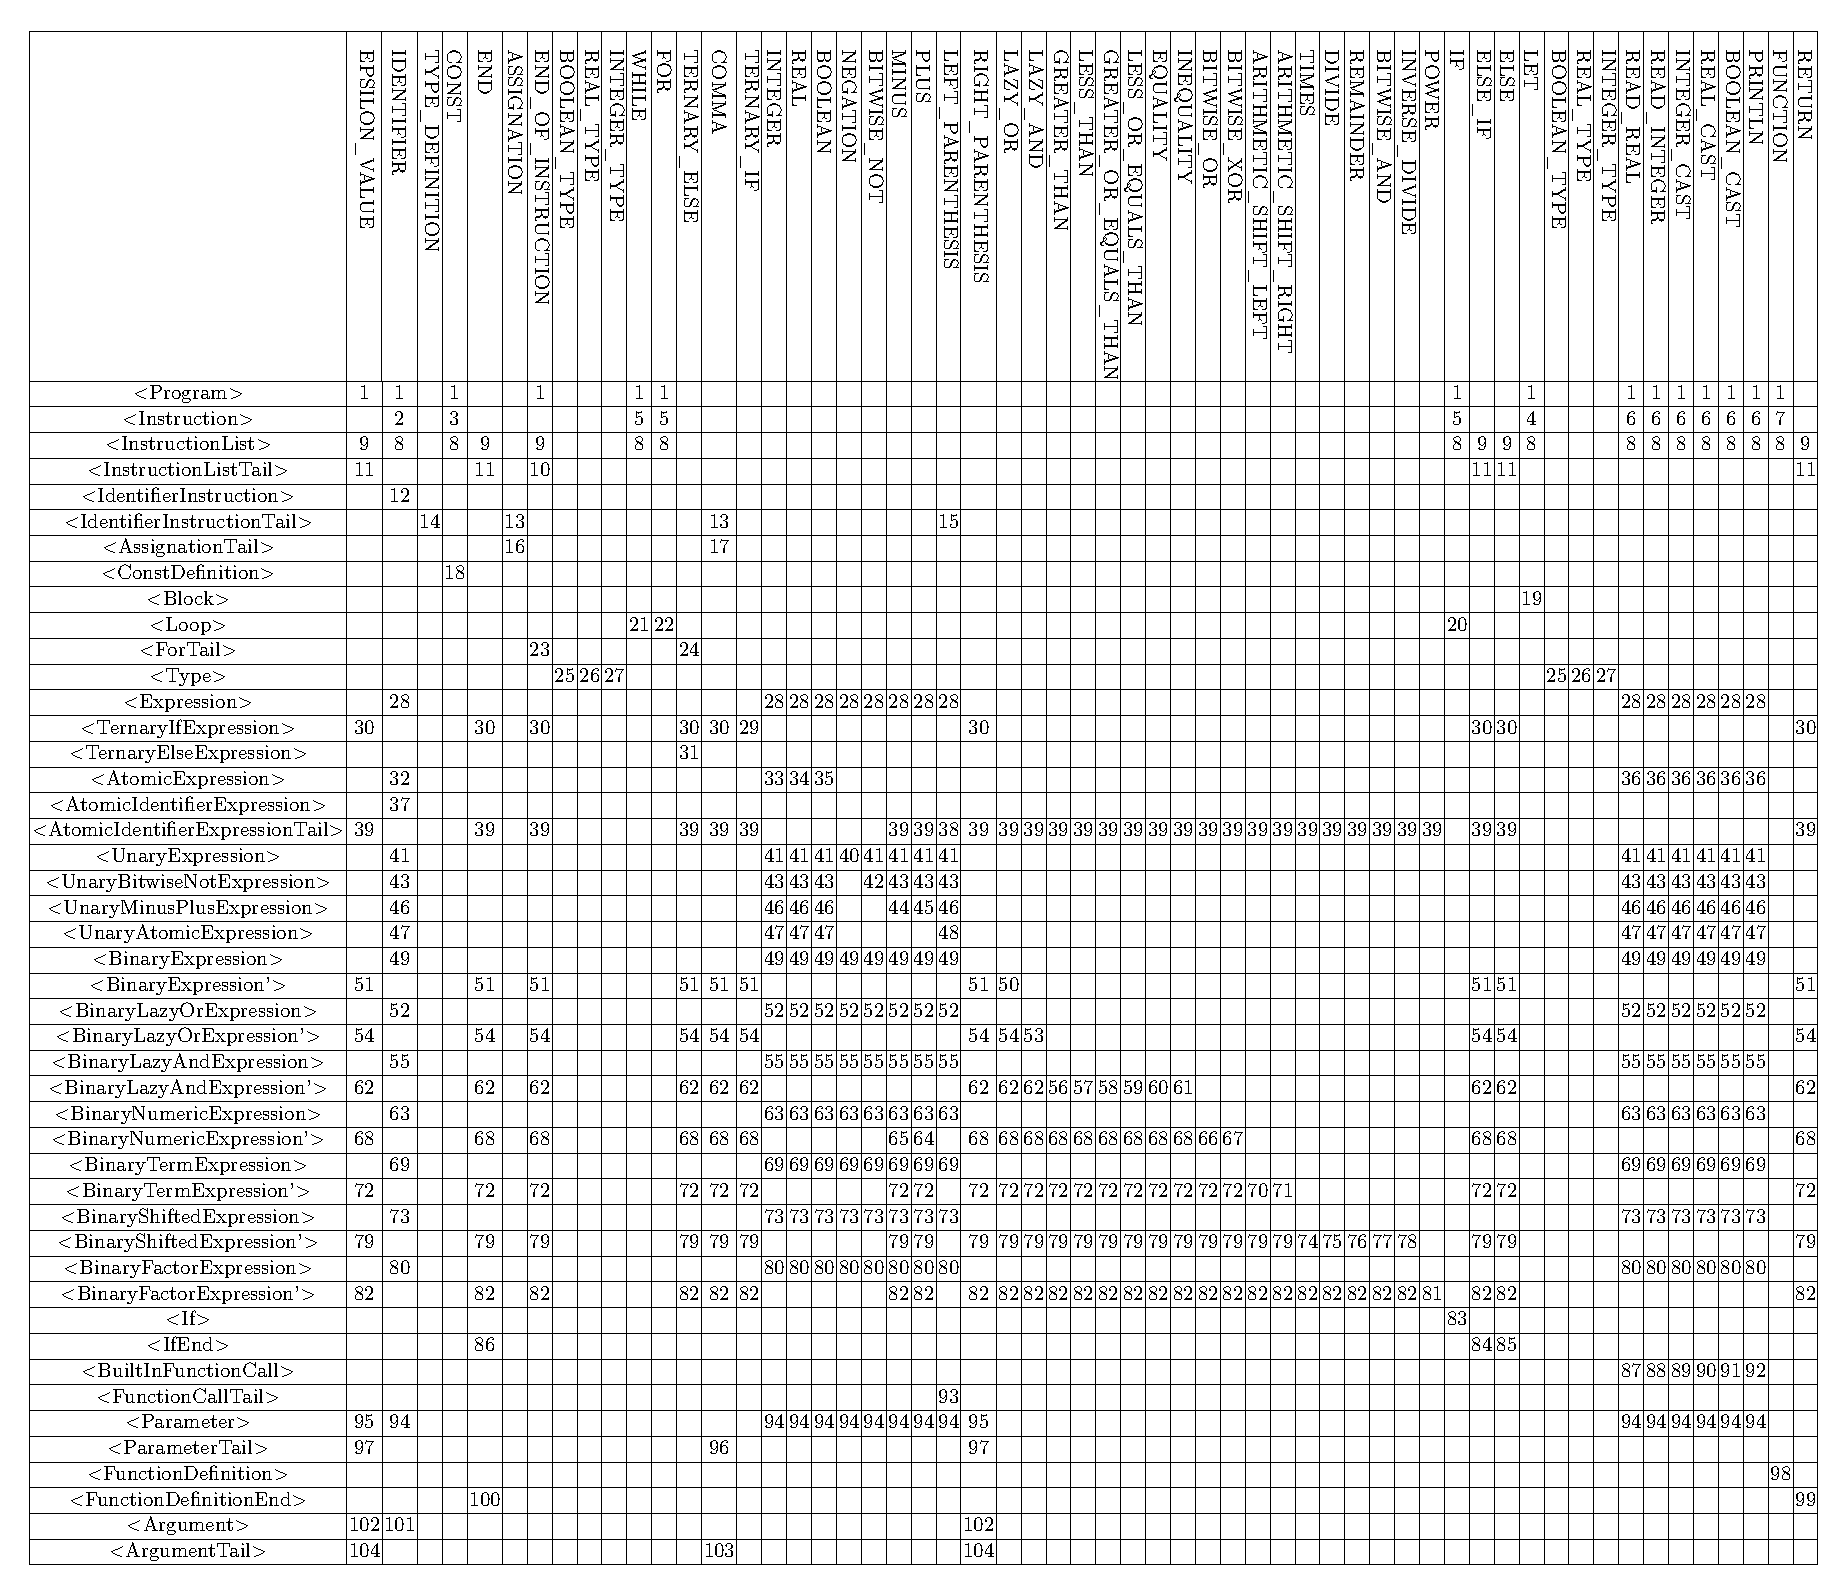
\includepdf[pages=1, angle=90]{AT.pdf}
\end{figure}

\end{document}
